% vim:spelllang=ru,en
\documentclass[a4paper,12pt,notitlepage,headsepline,pdftex]{scrartcl}

\usepackage{cmap} % чтобы работал поиск по PDF
\usepackage[T2A]{fontenc}
\usepackage[utf8]{inputenc}
\usepackage[english,russian]{babel}
\usepackage{concrete}
\usepackage{cite}
\usepackage{url}

\usepackage{textcase}
\usepackage[pdftex]{graphicx}

\usepackage{lscape}

\pdfcompresslevel=9 % сжимать PDF
\usepackage{pdflscape} % для возможности альбомного размещения некоторых страниц
\usepackage[pdftex]{hyperref}
% настройка ссылок в оглавлении для pdf формата
\hypersetup{unicode=true,
            pdftitle={ПОЭВМ Лаба №5},
            pdfauthor={Погода Михаил},
            pdfcreator={pdflatex},
            pdfsubject={},
            pdfborder    = {0 0 0},
            bookmarksopen,
            bookmarksnumbered,
            bookmarksopenlevel = 2,
            pdfkeywords={},
            colorlinks=true, % установка цвета ссылок в оглавлении
            citecolor=black,
            filecolor=black,
            linkcolor=black,
            urlcolor=blue}

\usepackage{amsmath}
\usepackage{amssymb}
\usepackage{moreverb}
\usepackage{indentfirst}
\usepackage{misccorr}

\usepackage{xtab}
\usepackage{nccfoots}
\usepackage{listings}

\lstloadlanguages{C++}
\lstset{language=C++,basicstyle=\scriptsize,frame=tb,commentstyle=\itshape,stringstyle=\bfseries,extendedchars=false}
\begin{document}
\begin{titlepage}
  \begin{center}
    \large
    \MakeUppercase{Министерство образования и науки,}

    \MakeUppercase{молодёжи и спорта Украины}

    \mbox{\MakeUppercase{Национальный технический университет Украины}}

    \MakeUppercase{,,Киевский политехнический институт''}

    \addvspace{6pt}

    \normalsize
    Кафедра прикладной математики

    \vfill

    \textbf{Отчёт}

    Лабораторная работа \No 5

    по дисциплине ,,Программное обеспечение ЭВМ''

    \emph{,,Линейное программирование''}
  \end{center}

  \vfill

  \noindent
  \begin{minipage}{0.3\textwidth}
    Выполнил

    студент группы КМ-92

    Погода~М.\,В.
  \end{minipage}
  \hfill
  \begin{minipage}{0.4\textwidth}
    Проверила:

    Ковальчук"=Химюк~Л.\,А.
  \end{minipage}
  \vfill

  \begin{center}
    КИЕВ

    2012
  \end{center}
\end{titlepage}
\tableofcontents
\newpage
\section{Постановка задачи}
  Предприятие выпускает 2 вида изделий: $P_1$ и $P_2$, каждое из кооторых
  проходит последовательную обработку на станках типов $T_1, T_2$ и $T_3$.
  Запас мощностей станков, т.\,е. рабочее время станка, составляет
  соответственно $B_1, B_2$ и $B_3$ единиц времени.
  При реализации одно изделие $P_i$ приносит предприятию $C_i$ единиц прибыли.

  \textit{Требуется} составить такой план загрузки станков, при котором
  предприятие получит максимальную прибыль.
\section{Входные данные}
  \hfill\emph{Вариант~4}
  \begin{table}[h]
    \centering
    \begin{tabular}{|c|cc|}
      \hline
        & $P_1$ & $P_2$\\
      \hline
      $T_1$ & 2 & 3\\
      $T_2$ & 3 & 1\\
      $T_3$ & 0 & 1\\
      \hline
    \end{tabular}
    \caption{Продолжительность обработки изделия на станке}
    \label{tab:duration}
  \end{table}

  \begin{table}[h!]
    \centering
    \begin{tabular}{|cc|}
      \hline
      $C_1$ & $C_2$\\
      \hline
      11 & 9\\
      \hline
    \end{tabular}
    \caption{Доход от реализации изделия}
    \label{tab:income}
  \end{table}

  \begin{table}[h!]
    \centering
    \begin{tabular}{|c|c|}
      \hline
      $T_1$ & 20\\
      $T_2$ & 27\\
      $T_3$ & 30\\
      \hline
    \end{tabular}
    \caption{Запас мощности станков}
    \label{tab:reserve}
  \end{table}

  \newpage
\section{Теоретические сведения}
  После формализации задача примет вид:
  \begin{equation}
    \label{eq:maxf}
    \max f\left( x_1, x_2 \right) = 11 x_1 + 9 x_2
  \end{equation}
  При ограничениях
  \begin{equation}
    \label{eq:cases}
    \begin{cases}
      2 x_1 + 3 x_2 &\leqslant 20\\
      3 x_1 + \hspace{0.2cm}x_2 &\leqslant 27\\
      \hspace{1.3cm}  x_2 &\leqslant 30
    \end{cases}
  \end{equation}
  \newpage
\section{Решение}
  Максимум функции, указанной в~\eqref{eq:maxf} при условиях~\eqref{eq:cases},
  достигается при $x_1 = 10, x_2 = 0$  и равен 110.

  Точное решение, полученное в Maxima CAS\footnote{Computer algebra system},
  полностью совпадает с данным решением.

\section{Описание программы}
  Программа написана на языке C++ с использованием библиотеки
  Qt\footnote{\url{http://qt-project.org}}.
  Программа ищет решение задачи линейного программирования симплекс"=методом.

  Пользователь имеет возможность поменять параметры линейного
  программирования.

  В результате работы программа выводит полученное оптимальное решение, а
  также значения, при которых оно достигается.
  \newpage
\section{Блок"=схема алгоритма}
  \begin{figure}[h!]
    \begin{center}
      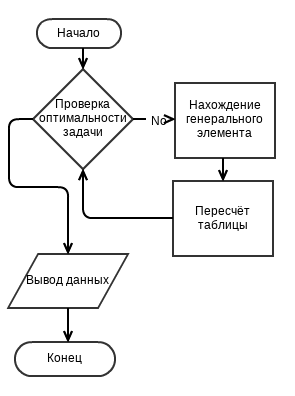
\includegraphics[scale=0.60]{flowchart.png}
    \end{center}
    \caption{Блок"=схема алгоритма}
    \label{fig:flowchart}
  \end{figure}
  \newpage
\section{Выводы}
  При выполнении данной лабораторной работы был реализован симплекс"=метод,
  который позволяет решать задачи линейного программирования.

  Так как симплекс метод является точным методом, полученное решение не
  отличается от реального.
  \newpage
\section{Приложения}
  \subsection{Графическая форма приложения}
    \begin{figure}[h!]
      \begin{center}
        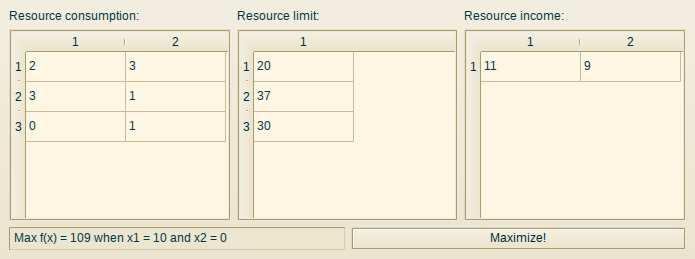
\includegraphics[width=\textwidth]{scr.png}
      \end{center}
      \caption{Графическая форма приложения}
      \label{fig:gui}
    \end{figure}
  \subsection{Исходные тексты}
    \subsubsection{CMakeLists.txt}
      \lstinputlisting{/home/projects/apps-for-computing/lab5/CMakeLists.txt}
    \subsubsection{lab5\_widget.hxx}
      \lstinputlisting{/home/projects/apps-for-computing/lab5/lab5_widget.hxx}
    \subsubsection{lab5\_widget.cxx}
      \lstinputlisting{/home/projects/apps-for-computing/lab5/lab5_widget.cxx}
\end{document}
